%!TEX root = ../Thesis.tex

\section{Use-Cases}

Im nachfolgenden sind die Use-Cases des Programm dargestellt (Siehe \cref{fig:usecases}).
Diese sind den Projektvorgaben entnommen.\footnote{Vgl. \cite{Vorgaben2020}}

\begin{figure}[hbt]\label{usecase}
\centering
\begin{minipage}[t]{1\textwidth}
    \caption{Use-Case Diagramm}
    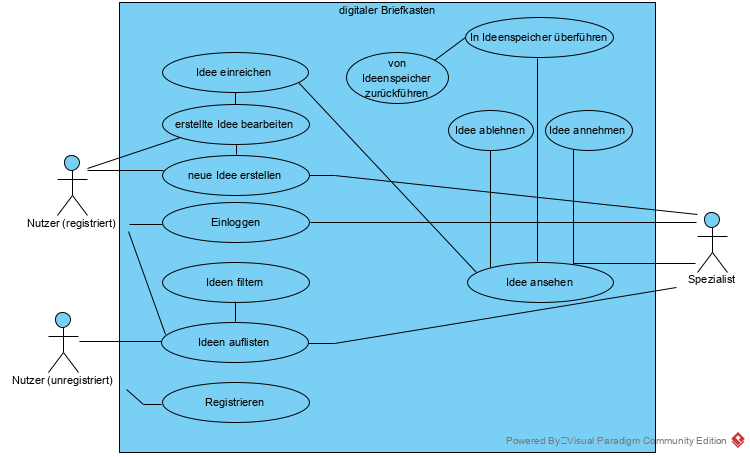
\includegraphics[width=1\textwidth]{img/createAnAccountWithSpamMailAccountYouSucker.png}\\
    \source{Eigene Darstellung}
    \label{fig:usecases}
\end{minipage}
\end{figure}

Für das Use-Case Diagramm sind drei Rollen von Relevanz.
Zuerst der \texttt{unregistrierte Nutzer}, welche die Sicht des Programmes für die Öffentlichkeit repräsentiert.
Desweiteren der \texttt{eingeloggte Nutzer} der mehr Möglichkeiten hat, hierzu gehört auch der \texttt{Administrator}.
Dieser hat über die Möglichkeiten des Nutzers weitere administrative Rechte.\footnote{Der Admin ist als eigener Use-Case im Anhang dargestellt. Siehe Anhang \ref{Anhang-Admin} auf S.\pageref{Anhang-Admin}}
Jedoch besitzt er nicht die Rechte der dritten Rolle des \texttt{Spezialisten}.\\

Die Use-Cases lassen sich in zwei \enquote{Kern}-Kategorien unterteilen.
Das sind zum einen die \texttt{Account} bezogenen Use-Cases.\\
Hierzu gehören der Vorgang des Einloggens sowie der Registrierung.
Zu diesen ist anzumerken, dass Spezialisten sich lediglich einloggen können.
Durch ihre administrative Rolle werden diese durch den Administrator angelegt.\\
Zum anderen ist der zweite Use-Case die \texttt{Erstellung und Bewertung von Ideen}.\\
Eingereichte Ideen lassen sich durch alle Nutzer jeder Rolle einsehen und filtern. Darüber hinaus haben alle eingeloggten Nutzer die Möglichkeit Ideen zu erstellen, zu bearbeiten und zur Bewertung einzureichen.\\
Diese eingereichten Ideen werden durch Spezialisten bewertet oder gespeichert.

Desweiteren exisitiert die Möglichkeit für alle Nutzer dem Administrator der Plattform über ein Kontaktformular Nachrichten zu senden.\footnote{Das zugehörige Use-Case Diagramm findet sich im Anhang \ref{Anhang-Kontakt} auf S.\pageref{Anhang-Kontakt}}